\documentclass{standalone}
\usepackage{tikz}
\usetikzlibrary{patterns, positioning}


\begin{document}
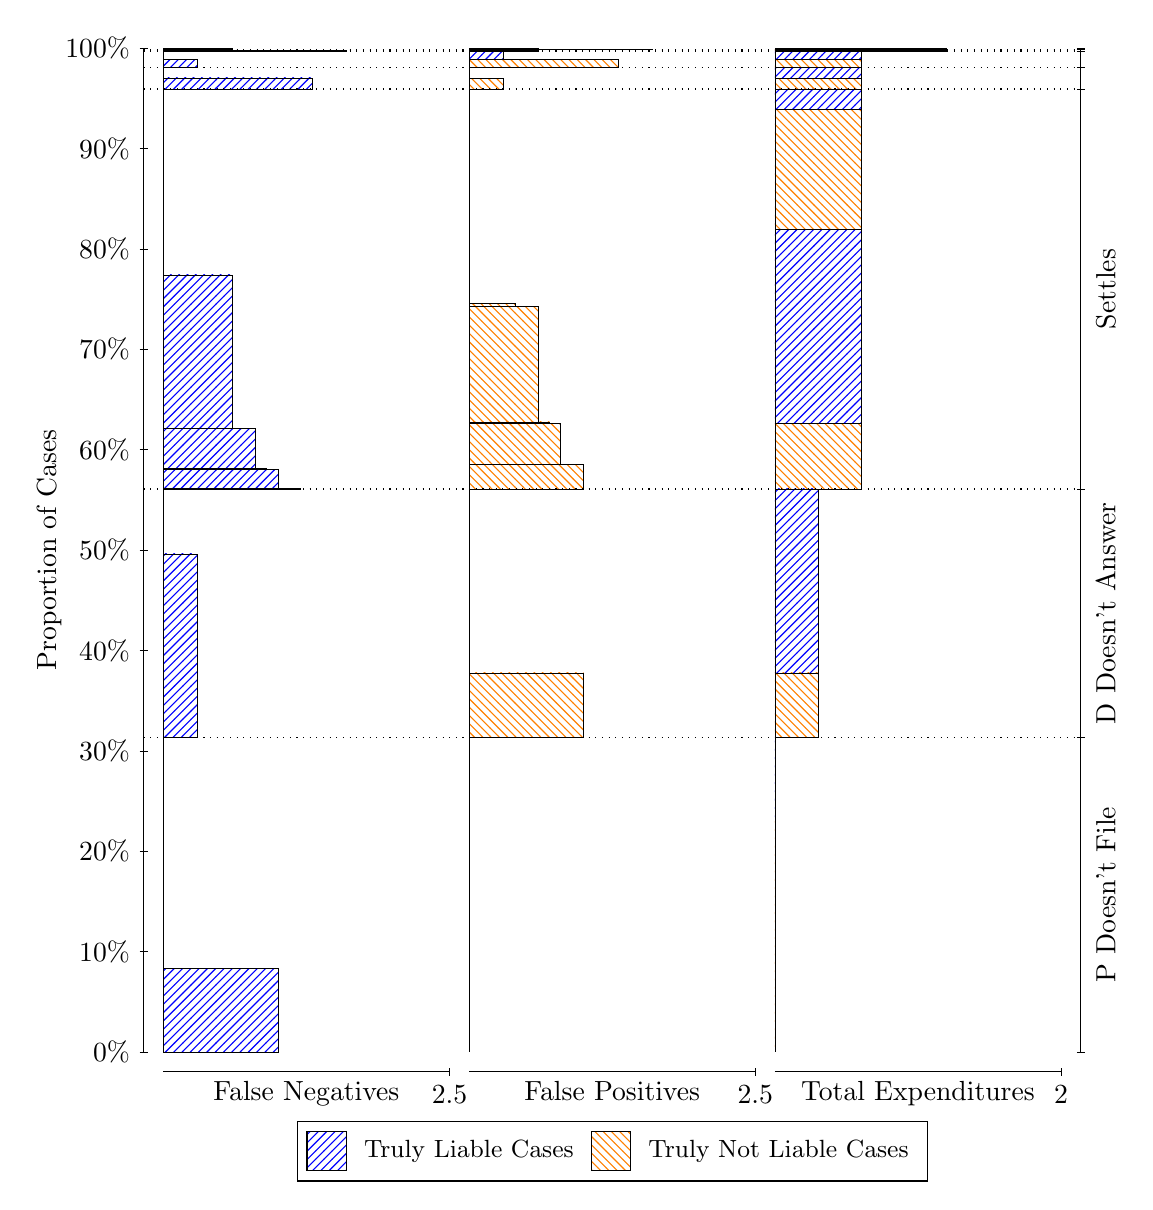
\begin{tikzpicture}
\draw[black, very thin] (1.5,1.75) -- (1.5,14.5);
\node[rotate=90, text=black, anchor=center] at (0.3, 8.125) {Proportion of Cases};
\draw[black, very thin] (1.45,1.75) -- (1.55,1.75);
\node[text=black, anchor=east] at (1.45, 1.75) {0\%};
\draw[black, very thin] (1.45,3.025) -- (1.55,3.025);
\node[text=black, anchor=east] at (1.45, 3.025) {10\%};
\draw[black, very thin] (1.45,4.3) -- (1.55,4.3);
\node[text=black, anchor=east] at (1.45, 4.3) {20\%};
\draw[black, very thin] (1.45,5.575) -- (1.55,5.575);
\node[text=black, anchor=east] at (1.45, 5.575) {30\%};
\draw[black, very thin] (1.45,6.85) -- (1.55,6.85);
\node[text=black, anchor=east] at (1.45, 6.85) {40\%};
\draw[black, very thin] (1.45,8.125) -- (1.55,8.125);
\node[text=black, anchor=east] at (1.45, 8.125) {50\%};
\draw[black, very thin] (1.45,9.4) -- (1.55,9.4);
\node[text=black, anchor=east] at (1.45, 9.4) {60\%};
\draw[black, very thin] (1.45,10.675) -- (1.55,10.675);
\node[text=black, anchor=east] at (1.45, 10.675) {70\%};
\draw[black, very thin] (1.45,11.95) -- (1.55,11.95);
\node[text=black, anchor=east] at (1.45, 11.95) {80\%};
\draw[black, very thin] (1.45,13.225) -- (1.55,13.225);
\node[text=black, anchor=east] at (1.45, 13.225) {90\%};
\draw[black, very thin] (1.45,14.5) -- (1.55,14.5);
\node[text=black, anchor=east] at (1.45, 14.5) {100\%};

\draw[black, very thin] (13.4,1.75) -- (13.4,14.5);
\draw[black, very thin] (13.35,1.75) -- (13.45,1.75);
\node[anchor=west] at (13.35, 1.75) {};
\draw[black, very thin] (13.35,5.7406) -- (13.45,5.7406);
\node[anchor=west] at (13.35, 5.7406) {};
\draw[black, very thin] (13.35,8.8999) -- (13.45,8.8999);
\node[anchor=west] at (13.35, 8.8999) {};
\draw[black, very thin] (13.35,13.98) -- (13.45,13.98);
\node[anchor=west] at (13.35, 13.98) {};
\draw[black, very thin] (13.35,14.254) -- (13.45,14.254);
\node[anchor=west] at (13.35, 14.254) {};
\draw[black, very thin] (13.35,14.462) -- (13.45,14.462);
\node[anchor=west] at (13.35, 14.462) {};
\draw[black, very thin] (13.35,14.48) -- (13.45,14.48);
\node[anchor=west] at (13.35, 14.48) {};
\draw[black, very thin] (13.35,14.5) -- (13.45,14.5);
\node[anchor=west] at (13.35, 14.5) {};

\draw[black, very thin, pattern color=blue, pattern=north east lines] (1.75,1.75) rectangle (3.2033,2.8083);
\draw[black, very thin, pattern color=orange, pattern=north west lines] (1.75,2.8083) rectangle (1.75,5.7406);
\draw[black, very thin, pattern color=blue, pattern=north east lines] (1.75,5.7406) rectangle (2.186,8.075);
\draw[black, very thin, pattern color=orange, pattern=north west lines] (1.75,8.075) rectangle (1.75,8.8999);
\draw[black, very thin, pattern color=blue, pattern=north east lines] (1.75,8.8999) rectangle (3.494,8.911);
\draw[black, very thin, pattern color=blue, pattern=north east lines] (1.75,8.911) rectangle (3.2033,9.1472);
\draw[black, very thin, pattern color=blue, pattern=north east lines] (1.75,9.1472) rectangle (3.058,9.1574);
\draw[black, very thin, pattern color=blue, pattern=north east lines] (1.75,9.1574) rectangle (2.9127,9.6715);
\draw[black, very thin, pattern color=blue, pattern=north east lines] (1.75,9.6715) rectangle (2.622,11.619);
\draw[black, very thin, pattern color=orange, pattern=north west lines] (1.75,11.619) rectangle (1.75,13.98);
\draw[black, very thin, pattern color=blue, pattern=north east lines] (1.75,13.98) rectangle (3.6393,14.122);
\draw[black, very thin, pattern color=orange, pattern=north west lines] (1.75,14.122) rectangle (1.75,14.254);
\draw[black, very thin, pattern color=blue, pattern=north east lines] (1.75,14.254) rectangle (2.186,14.355);
\draw[black, very thin, pattern color=orange, pattern=north west lines] (1.75,14.355) rectangle (1.75,14.462);
\draw[black, very thin, pattern color=blue, pattern=north east lines] (1.75,14.462) rectangle (4.0753,14.468);
\draw[black, very thin, pattern color=orange, pattern=north west lines] (1.75,14.468) rectangle (1.75,14.48);
\draw[black, very thin, pattern color=blue, pattern=north east lines] (1.75,14.48) rectangle (2.622,14.494);
\draw[black, very thin, pattern color=orange, pattern=north west lines] (1.75,14.494) rectangle (1.75,14.5);
\draw[black, very thin, pattern color=orange, pattern=north west lines] (5.6333,1.75) rectangle (5.6333,4.6823);
\draw[black, very thin, pattern color=blue, pattern=north east lines] (5.6333,4.6823) rectangle (5.6333,5.7406);
\draw[black, very thin, pattern color=orange, pattern=north west lines] (5.6333,5.7406) rectangle (7.0867,6.5654);
\draw[black, very thin, pattern color=blue, pattern=north east lines] (5.6333,6.5654) rectangle (5.6333,8.8999);
\draw[black, very thin, pattern color=orange, pattern=north west lines] (5.6333,8.8999) rectangle (7.0867,9.2082);
\draw[black, very thin, pattern color=orange, pattern=north west lines] (5.6333,9.2082) rectangle (6.796,9.7325);
\draw[black, very thin, pattern color=orange, pattern=north west lines] (5.6333,9.7325) rectangle (6.6507,9.7528);
\draw[black, very thin, pattern color=orange, pattern=north west lines] (5.6333,9.7528) rectangle (6.5053,11.22);
\draw[black, very thin, pattern color=orange, pattern=north west lines] (5.6333,11.22) rectangle (6.2147,11.261);
\draw[black, very thin, pattern color=blue, pattern=north east lines] (5.6333,11.261) rectangle (5.6333,13.98);
\draw[black, very thin, pattern color=orange, pattern=north west lines] (5.6333,13.98) rectangle (6.0693,14.111);
\draw[black, very thin, pattern color=blue, pattern=north east lines] (5.6333,14.111) rectangle (5.6333,14.254);
\draw[black, very thin, pattern color=orange, pattern=north west lines] (5.6333,14.254) rectangle (7.5227,14.36);
\draw[black, very thin, pattern color=blue, pattern=north east lines] (5.6333,14.36) rectangle (6.0693,14.462);
\draw[black, very thin, pattern color=orange, pattern=north west lines] (5.6333,14.462) rectangle (6.5053,14.474);
\draw[black, very thin, pattern color=blue, pattern=north east lines] (5.6333,14.474) rectangle (5.6333,14.48);
\draw[black, very thin, pattern color=orange, pattern=north west lines] (5.6333,14.48) rectangle (7.9587,14.486);
\draw[black, very thin, pattern color=blue, pattern=north east lines] (5.6333,14.486) rectangle (6.5053,14.5);
\draw[black, very thin, pattern color=orange, pattern=north west lines] (9.5167,1.75) rectangle (9.5167,4.6823);
\draw[black, very thin, pattern color=blue, pattern=north east lines] (9.5167,4.6823) rectangle (9.5167,5.7406);
\draw[black, very thin, pattern color=orange, pattern=north west lines] (9.5167,5.7406) rectangle (10.062,6.5654);
\draw[black, very thin, pattern color=blue, pattern=north east lines] (9.5167,6.5654) rectangle (10.062,8.8999);
\draw[black, very thin, pattern color=orange, pattern=north west lines] (9.5167,8.8999) rectangle (10.607,9.7325);
\draw[black, very thin, pattern color=blue, pattern=north east lines] (9.5167,9.7325) rectangle (10.607,12.194);
\draw[black, very thin, pattern color=orange, pattern=north west lines] (9.5167,12.194) rectangle (10.607,13.722);
\draw[black, very thin, pattern color=blue, pattern=north east lines] (9.5167,13.722) rectangle (10.607,13.98);
\draw[black, very thin, pattern color=orange, pattern=north west lines] (9.5167,13.98) rectangle (10.607,14.111);
\draw[black, very thin, pattern color=blue, pattern=north east lines] (9.5167,14.111) rectangle (10.607,14.254);
\draw[black, very thin, pattern color=orange, pattern=north west lines] (9.5167,14.254) rectangle (10.607,14.36);
\draw[black, very thin, pattern color=blue, pattern=north east lines] (9.5167,14.36) rectangle (10.607,14.462);
\draw[black, very thin, pattern color=orange, pattern=north west lines] (9.5167,14.462) rectangle (11.697,14.474);
\draw[black, very thin, pattern color=blue, pattern=north east lines] (9.5167,14.474) rectangle (11.697,14.48);
\draw[black, very thin, pattern color=orange, pattern=north west lines] (9.5167,14.48) rectangle (11.697,14.486);
\draw[black, very thin, pattern color=blue, pattern=north east lines] (9.5167,14.486) rectangle (11.697,14.5);
\draw[black, dotted] (1.5,5.7406) -- (13.4,5.7406);
\draw[black, dotted] (1.5,8.8999) -- (13.4,8.8999);
\draw[black, dotted] (1.5,13.98) -- (13.4,13.98);
\draw[black, dotted] (1.5,14.254) -- (13.4,14.254);
\draw[black, dotted] (1.5,14.462) -- (13.4,14.462);
\draw[black, dotted] (1.5,14.48) -- (13.4,14.48);
\draw[black, very thin] (1.75,1.5) -- (5.3833,1.5);
\node[text=black, anchor=north] at (3.5667, 1.5) {False Negatives};
\draw[black, very thin] (5.3833,1.45) -- (5.3833,1.55);
\node[text=black, anchor=north] at (5.3833, 1.45) {2.5};

\draw[black, very thin] (5.6333,1.5) -- (9.2667,1.5);
\node[text=black, anchor=north] at (7.45, 1.5) {False Positives};
\draw[black, very thin] (9.2667,1.45) -- (9.2667,1.55);
\node[text=black, anchor=north] at (9.2667, 1.45) {2.5};

\draw[black, very thin] (9.5167,1.5) -- (13.15,1.5);
\node[text=black, anchor=north] at (11.333, 1.5) {Total Expenditures};
\draw[black, very thin] (13.15,1.45) -- (13.15,1.55);
\node[text=black, anchor=north] at (13.15, 1.45) {2};

\node[text=black, centered, rotate=90] at (13.72, 3.7453) {P Doesn't File};
\node[text=black, centered, rotate=90] at (13.72, 7.3202) {D Doesn't Answer};
\node[text=black, centered, rotate=90] at (13.72, 11.44) {Settles};





\draw (7.449999999999999,1.5) node[draw=none] (baseCoordinate) {};
\begin{scope}[align=center]
        \matrix[scale=0.5, draw=black, below=0.5cm of baseCoordinate, nodes={draw}, column sep=0.1cm]{
            \node[rectangle, draw, minimum width=0.5cm, minimum height=0.5cm, pattern color=blue, pattern=north east lines] {}; &
            \node[draw=none, font=\small, text=black] (B) {Truly Liable Cases}; &
            \node[rectangle, draw, minimum width=0.5cm, minimum height=0.5cm, pattern color=orange, pattern=north west lines] {}; &
            \node[draw=none, font=\small, text=black] (B) {Truly Not Liable Cases}; \\
            };
\end{scope}

\end{tikzpicture}
\end{document}